\documentclass{article}[12pt]
\usepackage{authblk}
\usepackage{subfig}
\usepackage[T1]{fontenc}
\usepackage{lmodern}
\usepackage{lineno}
\usepackage[nottoc,numbib]{tocbibind}
\usepackage{enumitem}
\usepackage{subcaption}
\usepackage[letterpaper, portrait, margin=1in]{geometry}
\usepackage{graphicx} % Required for inserting images
\usepackage[toc,page]{appendix}


\usepackage{amsmath}

\usepackage{needspace}
\usepackage{setspace}

\usepackage[american]{babel}

\usepackage{csquotes}
\usepackage[style=apa,sortcites=true,sorting=nyt,backend=biber]{biblatex}
\DeclareLanguageMapping{american}{american-apa}
\addbibresource{Bibliograph.bib}
\usepackage{setspace}
\doublespacing
	
\usepackage{lineno}
\linenumbers
\needspace{1\baselineskip}
\usepackage[colorlinks,allcolors=black]{hyperref}

\title{Stats \& Stumps: Using Machine Learning to Predict T20I Matches with Player and Venue Data}
\author[1]{Archith Sharma}
\date{}

\affil[1]{Texas Academy of Mathematics and Science}

\begin{document}

\maketitle
\begin{abstract}
Cricket is gaining popularity worldwide rapidly, and at the front is the newest format of the game, Twenty20 Internationals (T20I), and big data. This project attempts to predict cricket match outcomes using player-level performance metrics and machine learning models. A dataset of 1,029 T20I matches was analyzed, with player-level features engineered from batting and bowling statistics such as runs, strike rate, boundaries, wickets, economy rate, and maiden overs. These features were normalized by ground-specific scoring rates to account for venue effects. Four modeling approaches were compared: a simple heuristic based on total player impact, logistic regression with regularization, random forests, and support vector machines (SVMs). All models were implemented in \texttt{R} using packages such as \texttt{glmnet} and \texttt{e1071}. Logistic regression achieved the highest test accuracy of 70.24\%, balancing predictive performance with model interpretability. The final model was used to generate win probabilities for both past and unseen matches, including the 2024 T20 World Cup Final (India vs South Africa) and a March 2025 match between New Zealand and Pakistan. These predictions reflect tight contests and demonstrate the model's ability to quantify match uncertainty. Overall, the project illustrates how venue-adjusted, player-level impact metrics can enable robust and interpretable match outcome prediction and player comparison in international T20 cricket.
\end{abstract}
\textit{Keywords:} \\
T20I, Cricket, Machine Learning, Player Impact, Cricket Analytics, Venue Adjustment, Regression
\\
\\
GitHub Code for Data Processing, Figure Generation and Analysis, Modeling: \\ \href{https://github.com/ArchithSharma/CricketPredictions}{https://github.com/ArchithSharma/CricketPredictions}

\pagebreak
\begin{onehalfspacing}
\tableofcontents
\end{onehalfspacing}
\pagebreak
\section{Introduction}

Cricket is a bat-and-ball sport that originated in England and has grown into one of the most popular sports worldwide, particularly in countries like India, Australia, South Africa, and Pakistan. Played between two teams of 11 players each, the game involves batting, bowling, and fielding, with the primary objective being to score more runs than the opposing team. Cricket is played in different formats, ranging from the traditional five-day Test matches to the fast-paced Twenty20 (T20) format.

T20 cricket, the shortest and most explosive format of the game, revolutionized the sport with its fast-paced action and entertainment value. Each team gets a maximum of 20 overs (120 balls) to bat, encouraging aggressive stroke play, quick scoring, and strategic bowling. Since its official introduction in 2003, T20 cricket has gained massive popularity, leading to global tournaments such as the ICC T20 World Cup and franchise-based leagues such as the Indian Premier League (IPL) and the Big Bash League (BBL). With its thrilling finishes, power-hitting, and emphasis on adaptability, T20 cricket has attracted a new generation of fans while maintaining the essence of the sport.

The rise of predictive analytics in cricket has closely coincided with the rapid growth of the T20 format. With T20 matches fast-paced and often decided by fine margins, teams, analysts, and betting markets have increasingly turned to data-driven approaches to gain a competitive edge. The shorter format requires quick decision making, making real-time data analysis and predictive modeling crucial to optimize team strategies, player selection, and match predictions.

In this paper, a unique approach will be taken that focuses on a new impact factor (IF) of players for both batting and bowling, in addition to consideration of match venues. These factors will then be used to train 3 types of models commonly used in sports prediction: Regularized logistic regression, random forest classifier, and support vector machines (SVMs), with high test set accuracies of 67 - 70\%. \parencite{vistro_2019}

The paper is organized as follows. Section 2 (Materials and Methods) will explore the Cricinfo dataset and derive the impact factor used for batting and bowling, along with a ground-based scaling to account for different venues. Afterwards, multiple models are tested on the adjusted comprehensive impact factors. Section 3 shows the accuracy percentages of the models along with its prediction on select matches. Section 4 and 5 analyze the impact factor for different players and venues, followed by a discussion of the models and some conclusions/limitations. There are two appendices, the first containing figures generated that are used in the analysis and the code used (\ref{appendix:vis}), and the second containing a definition of common cricket terms used throughout the paper and the test-playing nations list (\ref{appendix:terms}).

\section{Materials and Methods}

All data pre-processing, analysis and modeling was performed in R. \parencite{r_software} See Appendix \ref{appendix:vis1} to locate the code used on GitHub and regenerate the figures.

\subsection{Description of Data}
\begin{figure}[!h]
    \centering
    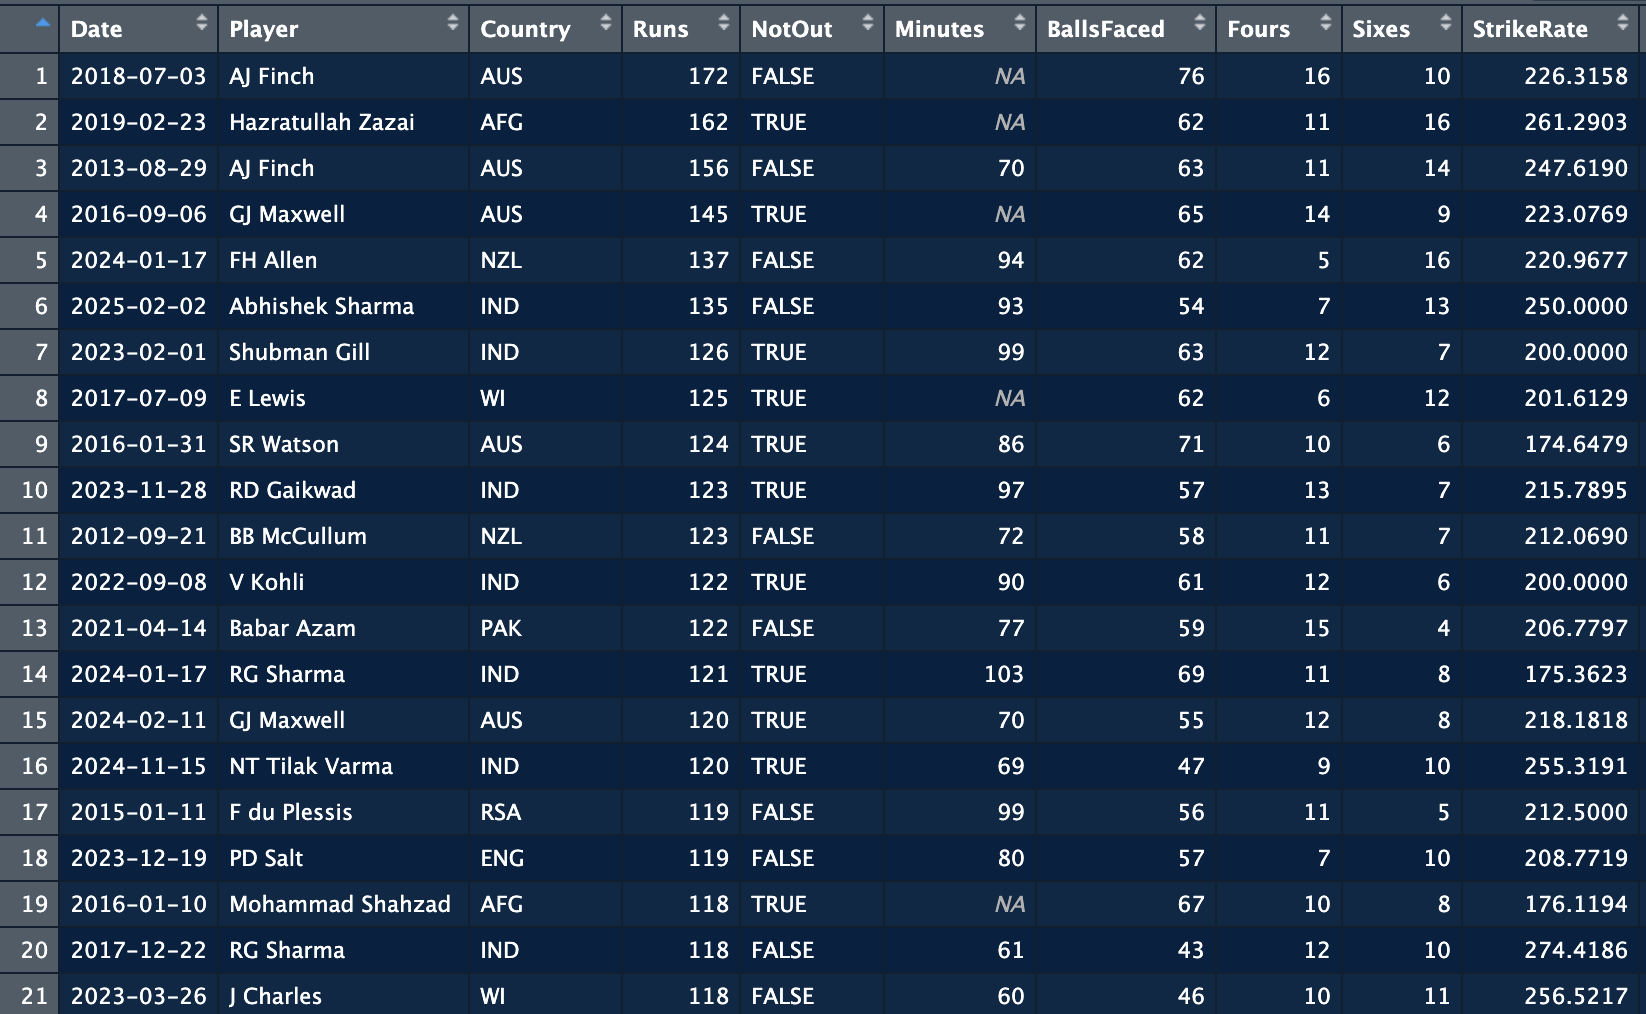
\includegraphics[width=0.5\linewidth]{batting_data.png}
    \caption{Batting Data}
    \label{fig:batting_data}
\end{figure}

 The data is taken from ESPN Cricinfo, a reputable source containing in-depth statistics on all T20Is played and the players themselves. \parencite{espn_2025_espncricinfo} To access the data in R, the \texttt{cricketdata} package made by Rob Hyndman \parencite{cricketdata} was used to access the Statsguru data in R as a dataframe. A screenshot of the batting dataframe is shown above in Figure \ref{fig:batting_data}.

The data is then filtered to only include T20Is between the test-playing full ICC members, defined in Appendix \ref{appendix:list}. The data is also joined by match to determine the total impact factor of teams in their matches, both bowling and batting.

\subsection{Derivation of Impact Factor}

At the core of this analysis is the novel impact factor used in comparing batting and bowling impacts. To determine the formula for batting and bowling impact, correlation to the target metric between the total impact of both teams was prioritized in addition to similarity in the distribution of the impact factors each game.

The impact factor was manually tuned to a quantity that sufficiently addressed both criteria. They are defined below in Equations \ref{eq1} and \ref{eq2}:

\subsubsection{Definition of Bat and Bowl Impact}
\begin{equation}
    \text{Batting Impact} = (R \times 0.125) + ((SR - 130) \times 0.025) + (4s \times 0.3) + (6s \times 0.5) - \text{OutPenalty}
    \label{eq1}
\end{equation}



\[
\begin{aligned}
\text{where:} \quad 
& R = \text{Runs scored} \\
& SR = \text{Strike rate} = \left( \frac{\text{Runs}}{\text{Balls Faced}} \times 100 \right) \\
& 4s = \text{Number of fours hit} \\
& 6s = \text{Number of sixes hit} \\
& \text{OutPenalty} = \text{Fixed penalty of 0.5 if the batter is dismissed}
\end{aligned}
\]

\[
\text{Example:}
\]
\[
\text{A batter scores } R = 40 \text{ runs off } 28 \text{ balls, hits } 3 \text{ fours, 2 sixes, and is dismissed.}
\]
\[
SR = \frac{40}{28} \times 100 \approx 142.86, \quad \text{OutPenalty} = 0.5
\]
\[
\text{Batting Impact} = (40 \times 0.125) + ((142.86 - 130) \times 0.025) + (3 \times 0.3) + (2 \times 0.5) - 0.5
\]
\[
= 5 + (12.86 \times 0.025) + 0.9 + 1.0 - 2.5 = 5 + 0.3215 + 0.9 + 1.0 - 0.5 \approx \textbf{6.72}
\]

\begin{equation}
    \text{Bowling Impact} = (W \times 3.25) + (M \times 3) - ((E - 7.4) \times 0.5)
    \label{eq2}
\end{equation}

\[
\begin{aligned}
\text{where:} \quad 
& W = \text{Number of wickets taken} \\
& M = \text{Number of maiden overs bowled} \\
& E = \text{Economy rate} = \left( \frac{\text{Runs Conceded}}{\text{Overs Bowled}} \right) \\
& 7.4 = \text{Baseline economy rate for adjustment} \\
& 0.5 = \text{Penalty per unit increase in economy above 7.4}
\end{aligned}
\]

\[
\text{Example:}
\]
\[
\text{A bowler takes } W = 2 \text{ wickets and a } E = 6.85 \text{ economy rate } 3 \text{ and has no maiden overs.}
\]
\[
\text{Bowling Impact} = (2 \times 3.25) + (0 * 3) - ((6.85 - 7.4) * 0.5) = 6.5 + 0.55 * 0.5 \approx \textbf{6.775}
\]

Both batting and bowling equations consider a baseline adjustment for strike rate and economy rate based on the average score of around 149 in T20Is. \parencite{statsguru_2025_total} Both example players did very well in their respective games and had high similar impacts of around 6.75, showing the relevance of the heuristic.

Afterwards, the batting and bowling impacts were grouped by their totals by game for each team. Afterwards, the differences between total impact factors are used as a heuristic to be correlated to the winner of the match (interpreted numerically as 1, 0). As can be seen in the code, the correlation value is 0.773 for 1029 T20Is, and the \(R^2\) is 0.598, approximately 0.6 which indicates high explainability.

\subsubsection{ANOVA and Histogram Validation of Bat/Bowl Similarity}
To validate the assumption that the distributions are similar, an analysis of variance (ANOVA) is performed by modeling the batting impacts on the bowling impacts and the result is displayed in Table \ref{tab:anova_results}. The p-value that is almost 0 shows that the distributions are very similar. In addition the visual validation of the histogram in Figure \ref{fig:imdist} shows how similar the total impact factors are, and that they can be used for modeling.
\begin{table}[!ht]
\centering
\begin{tabular}{lrrrrr}
\textbf{Term} & \textbf{Df} & \textbf{Sum Sq} & \textbf{Mean Sq} & \textbf{F value} & \textbf{Pr(>F)} \\
\hline
Total Bowling & 1 & 19376 & 19376 & 95.95 & $< 2 \times 10^{-16}$ \\
Residuals & 2068 & 417623 & 202 & & \\
\hline
\end{tabular}
\caption{ANOVA Results}
\label{tab:anova_results}
\end{table}
\begin{figure}[!h]
    \centering
    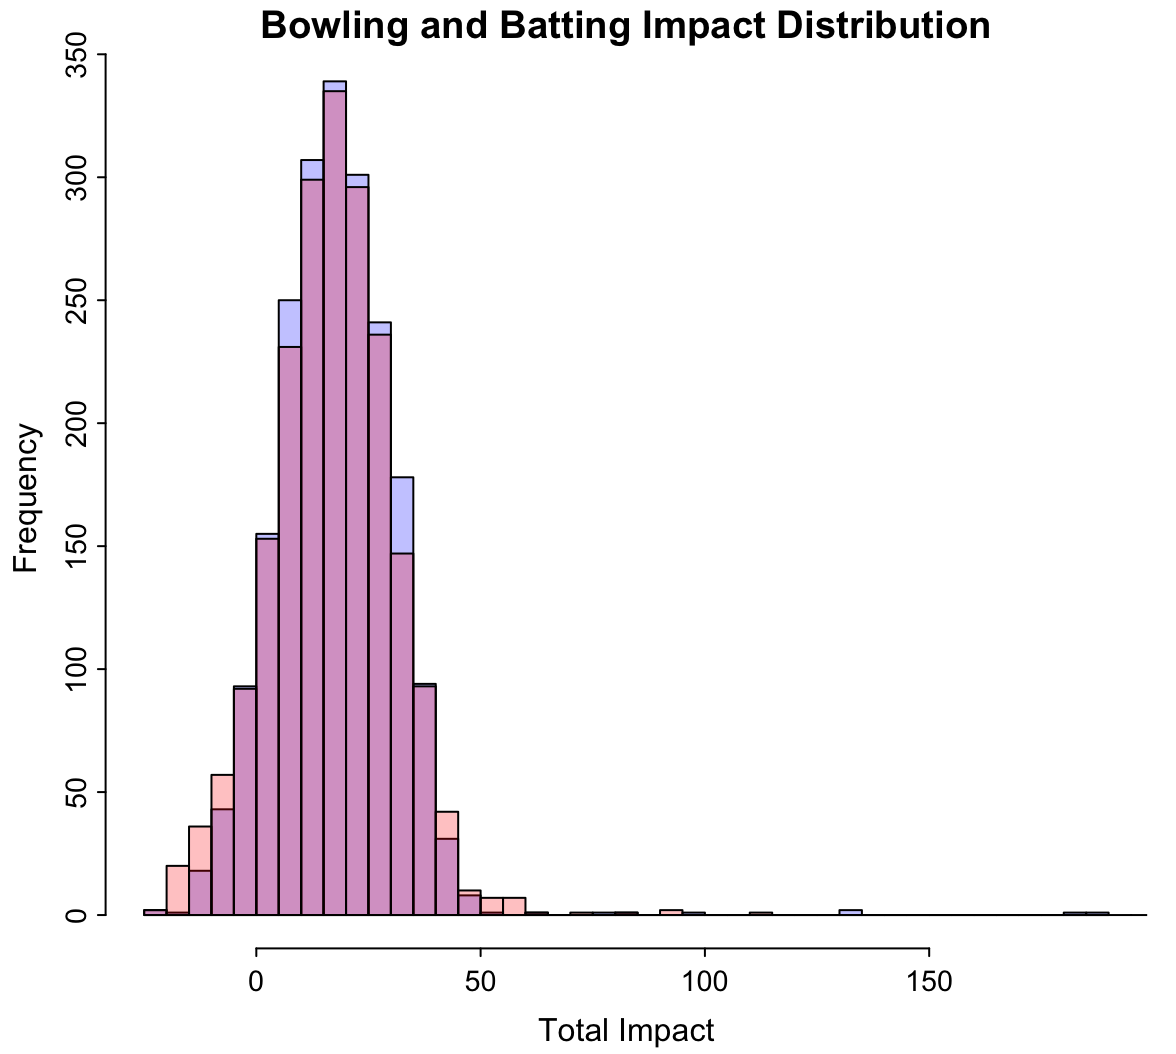
\includegraphics[width=0.5\linewidth]{impact_dist.png}
    \caption{Impact Distributions}
    \label{fig:imdist}
\end{figure}

\subsection{Determining Impact Factors to be used in Prediction}

In this study, the performance of players in a T20 match is evaluated through a series of factors that encompass both their batting and bowling abilities. The impact of each player is adjusted for various game-specific conditions, including venue-based adjustments and player rankings. Below, the rationale behind the decision-making process is outlined for each factor used in the calculation of player impact.

\subsubsection{Player Ratings and Impact Calculation}
Each player’s performance is assessed based on their batting and bowling ratings, which are derived from historical performance data. These ratings are extracted from the \texttt{player\_rankings\_2} dataset, which includes batting impact (\texttt{BatImpactperGame}) and bowling impact (\texttt{BowlImpactperGame}) for each player. These ratings reflect the overall contribution of a player to their team's performance in previous matches.

\subsubsection{Ground Buffs (Venue Factors)}
The performance of players is also adjusted based on the specific characteristics of the ground where the match is played. Each ground has unique attributes that can influence player performance, such as pitch conditions, weather, and altitude. The \texttt{venue\_factors} dataset provides ground-specific adjustments known as ``ground buffs''. These buffs are applied to both batting and bowling ratings to account for the venue’s impact on player performance. The following ground buffs are considered:
\begin{itemize}
    \item \textbf{Batting Buff} (\texttt{BattingScale2}): This factor adjusts the batting impact based on ground-specific conditions such as pitch type, boundary size, and weather.
    \item \textbf{Bowling Buff} (\texttt{BowlingScale2}): This factor adjusts the bowling impact based on similar ground conditions that affect how bowlers perform, including pitch conditions and boundary dimensions.
\end{itemize}

\subsubsection{Weighting by Player Ranking}
The weight assigned to each player's performance is influenced by their relative ranking in the team. Batting and bowling impact are adjusted according to player rankings:
\begin{itemize}
    \item \textbf{Batting Impact}: The top 8 batsmen (top and middle order) in the playing XI receive a weighted adjustment to their batting impact. The adjustment is proportional to the player’s ranking, with higher-ranked players receiving a greater weighting. The weight is calculated as a function of the player's position in the batting order, with later batsmen receiving lower weights to reflect their reduced role in the match.
    \item \textbf{Bowling Impact}: Similarly, the top 6 bowlers are given weighted adjustments to their bowling impact, based on their ranking. The adjustment is calculated in a similar manner, with higher-ranked bowlers receiving greater weight. The bottom bowlers are excluded from the impact calculation, as they are less likely to bowl in the match.
\end{itemize}

\subsubsection{Impact Per Game Adjustments to be used for prediction}
Once the initial ratings are adjusted for venue buffs and player rankings, the resulting impact values (\texttt{BatImpactperGame\_2} and \texttt{BowlImpactperGame\_2}) are calculated for each player. The calculations are performed iteratively for both teams, with batting and bowling impacts adjusted according to the above factors:
\begin{itemize}
    \item For batsmen, the weight is scaled according to their position in the batting order.
    \item For bowlers, a similar scaling is applied, with the most prominent bowlers receiving higher weights.
    \item The adjusted values for each player are stored and used to update the overall team impact.
\end{itemize}

\subsubsection{Calculation of Total Player Impact}
Finally, the adjusted batting and bowling impacts are compiled into a total impact score for each player. This score is split into batting and bowling impacts, with the first 8 players in the batting order contributing to the batting total, and the next 6 players contributing to the bowling total. The impact scores for each player from both teams are then consolidated into a total impact matrix, which represents the overall performance potential of the two teams based on individual player ratings and match conditions.

In summary, the impact factors in this methodology are derived from a combination of player rankings, ground-specific adjustments, and positional weights. These factors provide a comprehensive assessment of player performance, accounting for both individual ability and contextual factors, such as venue and team composition.

\subsection{Modeling}

To predict T20I match outcomes based on player-level performance metrics, several classification models were implemented and evaluated using a dataset where each match was represented by the total impact scores of 28 players (14 per team). As a baseline, a simple heuristic predicted the team with the higher cumulative impact score as the winner. This naive method yielded an accuracy of \textbf{64\%}, providing a benchmark for more advanced models.

A logistic regression model with elastic net regularization was trained using 5-fold cross-validation to tune the hyperparameters $\alpha$ and $\lambda$. \parencite{glmnet} To convert predicted probabilities into binary outcomes, optimal classification thresholds were selected by averaging the best thresholds across ROC curves in 10-fold cross-validation. \parencite{pROC_package} Repeating this process over 30 iterations, the logistic regression model achieved a maximum accuracy of \textbf{70.24\%}, outperforming the heuristic approach and all other models.

To enhance explainability, the coefficient weights were extracted from the logistic model. Features associated with top-order batters and key bowlers—such as the highest run scorers, highest strike rate performers, and wicket-takers—were consistently assigned large absolute coefficients, indicating their strong influence on match outcomes. Notably, impact scores from players in the top three batting positions had the greatest positive association with winning probability, while low-performing bowlers negatively influenced predicted outcomes. In addition, Batters 7-8 and Bowlers 5-6 had large coefficients, showing that the model respected lineup depth and all-rounder `X-factor' performances.

A random forest model with 500 trees was also tried, tuning the \texttt{mtry} parameter via internal 5-fold CV. This model achieved a maximum accuracy of \textbf{67.8\%}. Feature importance rankings from the random forest agreed with the logistic regression: early-order batters and strike bowlers had the greatest influence, though the non-linearity of the random forest also surfaced some interactions among lower-order players.

Lastly, a linear Support Vector Machine (SVM) was evaluated using a grid of cost values $C = 2^{-5}, \dots, 2^5$ and 5-fold cross-validation. \parencite{e1071} The best SVM model reached an accuracy of \textbf{69.7\%}, comparable to the logistic regression model.

Among all approaches, logistic regression offered the best performance while also allowing for direct interpretability through model coefficients. This suggests that linearly weighted combinations of individual player impacts can be powerful predictors of T20I match outcomes.



\section{Results}

\subsection{Player and Venue visualizations}
Now that the impact factors are clearly defined, they can be used to construct rankings of players by batting, bowling, or all-around play and venue factors. Similarly, teams can be ranked by their recent impact factors. The full visualizations of the Top 15 in Career Impact and Impact per Game for batsmen are found in Appendix \ref{appendix:vis2} containing Figures \ref{fig:career}, \ref{fig:bygame}, \ref{fig:allround}, and \ref{fig:venues}. All-rounders are defined as individuals in the top two-thirds of all players in batting and in the top 55th percentile of all players in bowling. The average venue impact was also min-max scaled to be used as a multiplier in the predictive modeling phase.

\subsection{Model Results}
The modeling results are organized below in Table \ref{tab:model-performance}.
\begin{table}[h!]
\centering
\begin{tabular}{|l|c|c|}
\hline
\textbf{Model} & \textbf{Mean Accuracy (\%)} & \textbf{95\% CI (\%)} \\
\hline
Heuristic (Total Impact Comparison) & 64.00 & [64.00, 64.00] \\
Logistic Regression (Elastic Net) & 68.32 & [66.42, 70.24] \\
Random Forest & 66.08 & [64.91, 67.80] \\
Support Vector Machine (Linear Kernel) & 67.42 & [65.53, 69.70] \\
\hline
\end{tabular}
\caption{Model performance based on mean accuracy and 95\% confidence intervals over 30 iterations}
\label{tab:model-performance}
\end{table}
\\
The following data in Table \ref{tab:select} is the model's output for select matches.
\begin{table}[h!]
\centering

\begin{tabular}{|l|c|l|l|}
\hline
\textbf{Match} & \textbf{Win Probability (\%)} & \textbf{Actual Winner} & \textbf{Margin} \\
\hline
IND vs RSA (T20 WC Final 2024) & IND: 50.46 & IND & 7 runs \\
NZ vs PAK (Unseen Match, March 26) & NZ: 55.45 & NZ & 8 wickets \\
BAN vs. WI Dec 19 2024 & BAN: 50.62 & BAN & 80 runs \\
IND vs. PAK Oct 23 2022 & IND: 64.5 & IND & 4 wickets \\
\hline
\end{tabular}
\caption{Predicted Win Probabilities and Actual Outcomes for Select T20I Matches}
\label{tab:select}
\end{table}



\section{Discussion}

\subsection{Analysis of Players and Venues}



\subsubsection{Player Analysis: Virat Kohli}

Virat Kohli is considered by many to be the world's best batsman, scoring the third most runs of all time and having the second most total hundreds. \parencite{espn_2025_espncricinfo2} However, many have shown doubt about his performances in the shortest format of the game, especially due to concerns about his strike rate. \parencite{toisportsdesk_2024_usually}

The impact factor method considers him one of the best, if not the best T20I batsmen despite his strike rate. He is ranked the best batsman by total career batting impact, while he finds the third spot in batting impact per game. His low strike rate is not enough of a hindrance due to the constant amount of runs he amasses. The impact factor is able to find value in his ability to facilitate the innings.

\subsubsection{Player Analysis: Ajantha Mendis}

Ajantha Mendis (labeled BAW Mendis) was a spinner for Sri Lanka between 2008 and 2014. He is the only player to take 6 wickets in a T20I twice, and also  won Emerging Player of the Year in 2008. Labelled a mystery spinner, when batsmen figured him out, he began to get hit all around the park. His biggest criticism was the lack of consistency, and he disappeared from Sri Lanka's XI in favor of Rangana Herath and other spinners. \parencite{cricbuzz_2025_ajantha}

The impact factor method has a shortcoming when considering a spinner like Mendis. Recent matches do not get weighted more since the model does not have a time factor, and high performances in a small dataset could push his impact as high as the third rank. To address it in model predictions, adding a random effect to the player impact based on the number of games played could make a difference. 

The theoretical framework would be that the more matches someone plays, the less deviation their impact score would have. Comparing Mendis and Kohli, where the former played one thirds the games the latter did, Mendis's variance parameter estimate would have 3 times the variance of Kohli's parameter and thus represent his inconsistency. Player dropping ensures the model stays representative regardless of consistency because inconsistent players tend to be dropped.

\subsubsection{Player Analysis: Glenn Maxwell}

Glenn Maxwell is considered the quintessential T20 player for the combination of his golden arm and power hitting. He can steal wickets from loose shots, and send loose deliveries 100 meters away. Most of his impact, however comes from batting. Unorthodox shots make him hard to stop when he gets going \parencite{espn_2023_afghanistan}, and his high batting impact scores and semi-decent bowling performances push him up the all-rounder list.

This is in contrast to someone like Wanindu Hasaranga higher on the list, who is a handy batsman lower in the order, but does most of his damage with the ball in his hands. Hardik Pandya is different from both, being middle-of-the-pack in bowling and batting. The impact factor method gives them high, yet roughly equal impacts which correspond to a correct aggregation.

\subsubsection{Venue Analysis: England vs. Subcontinent Venues}

The venue analysis by impact factor is mostly accurate to real-life ground impacts. 12 out of the top 20 best batting venues are located in either India or Pakistan, reflecting the popular opinion that many pitches in the subcontinent are batting paradises.

However, the grounds in England tend to be more balanced and favor the bowlers more. In total impact relative to batting, Lord's places 79th out of 105 venues. The famous slope at Lord's makes bowling relatively favorable as well. Southampton, The Oval and Headingley are all in the 60-70 range, reflecting England's moderate preference for bowling, showing that the scaling based on impact factor is an accurate measure of ground impacts.

\subsubsection{Team Rankings Based on Recent Matches}

Based on the impact factor, rankings based on the total accumulated impact can be constructed for the last 6 months. The data shows that India is far and away the most in-form team, followed by Australia and Afghanistan. South Africa and Pakistan are lower on the list, especially due to recent series losses to India and New Zealand, respectively. Ireland is also placed higher since they have not played the top teams in the last 6 months outside of Zimbabwe. However, overall, the list is an accurate representation of the current T20I landscape. 

\begin{figure}[!ht]
    \centering
    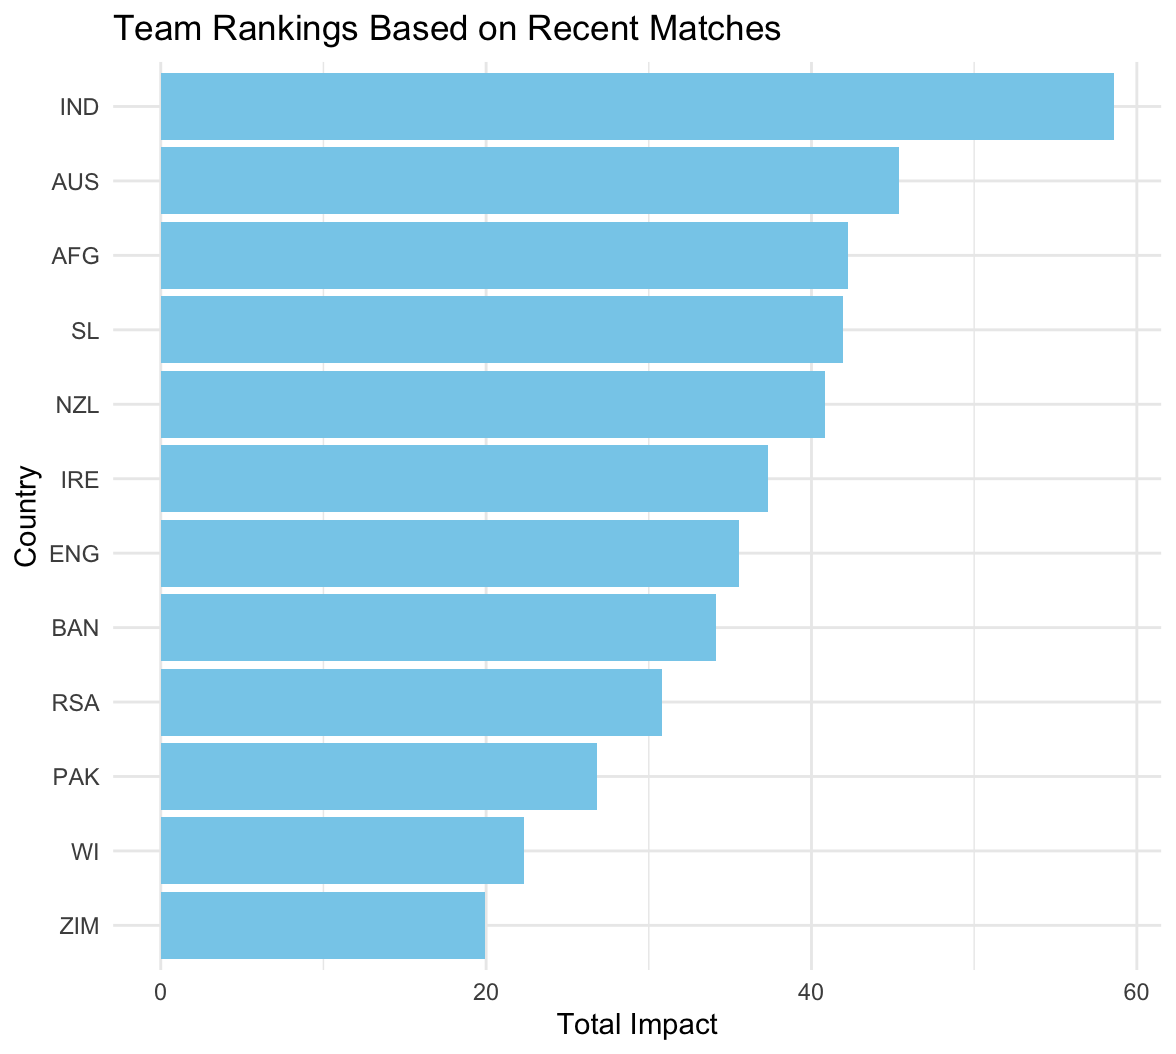
\includegraphics[width=0.5\linewidth]{team_rankings.png}
    \caption{Rankings based on performance for last 6 months}
    \label{fig:rankings}
\end{figure}


\subsection{Analysis of Models}

Four different approaches were tested for predicting T20I match outcomes: a simple heuristic model, logistic regression with regularization, random forests, and support vector machines (SVM). The heuristic model, which selects the team with the highest total player impact, achieved an accuracy of approximately 64\%, serving as a useful baseline. Logistic regression outperformed the others, reaching a maximum test accuracy of 70.24\%, with hyperparameter tuning and threshold optimization via cross-validation. Random forests and SVMs followed closely with peak accuracies of 67.8\% and 69.7\%, respectively.

Logistic regression was selected for final prediction due to its strong performance and interpretability. The model provides probabilistic outputs, allowing uncertainty to be quantified. For example, in the 2024 T20 World Cup Final between India and South Africa, the model assigned India a win probability of 50.46\%, reflecting an essentially even matchup which can be seen in the small result margin of 7 runs. Similarly, for the March 26 match between New Zealand and Pakistan, the model predicted a New Zealand win probability of 55.45\%, indicating a slight edge. 

These results suggest that logistic regression provides both competitive performance and actionable probabilities for match outcome predictions. Moreover, its explainability makes it suitable for understanding how individual player features contribute to team-level predictions.


\section{Conclusions}

This paper has been maximizing the value of a simple model in T20I prediction. More complex models can consider strategy with the toss before matches, as many pitches get better to bat on because of the dew in the night, meaning there is a significant advantage in batting second. \parencite{krishnaswamy_2022_the} In addition, recent player form can change the parameter passed into the logistic regression. For example, Virat Kohli was in a bad run of form during the T20 World Cup, only crossing 10 runs twice in the 7 matches before the final. Specific bowler-batsman combinations are not considered either, such as the Indian top order's issues with left arm pace bowlers.\parencite{iyer_2023_why} Overall, however, this paper's methods have had an accuracy of 70\% in predictions and an explainable impact factor that can be used to quantify team performance. This framework can streamline cricket analysis and objectively pit players and teams against each other through the power of data.

\section{Acknowledgements}

I would like to thank the Wharton Sports Analytics and Business Initiative for the opportunity to share my work, and especially Professor Adi Wyner for organizing the Wharton High School Data Science Competition, which sparked my interest in sports analytics. I am also grateful to the broader cricket analytics community, particularly ESPN Cricinfo and the open source contributors to the R Project. Special thanks to Dr. Rob J Hyndman, the creator of the \texttt{cricketdata} package, for enabling data-driven sports research. I would also like to thank my grandfather, Giridhara Govinda Rao for introducing me to the game of cricket and inspiring my love for it.









\clearpage
\addcontentsline{toc}{section}{References}

\printbibliography
\pagebreak

\begin{appendices}
\section{Player and Venue Visualizations, Code Used for Analysis and Figure Generation}
\label{appendix:vis}




\subsection{Player and Venue Diagrams}
\label{appendix:vis2}
\begin{figure}[!htb]
    \centering
    \subfloat[\centering Batting Career Impact]{{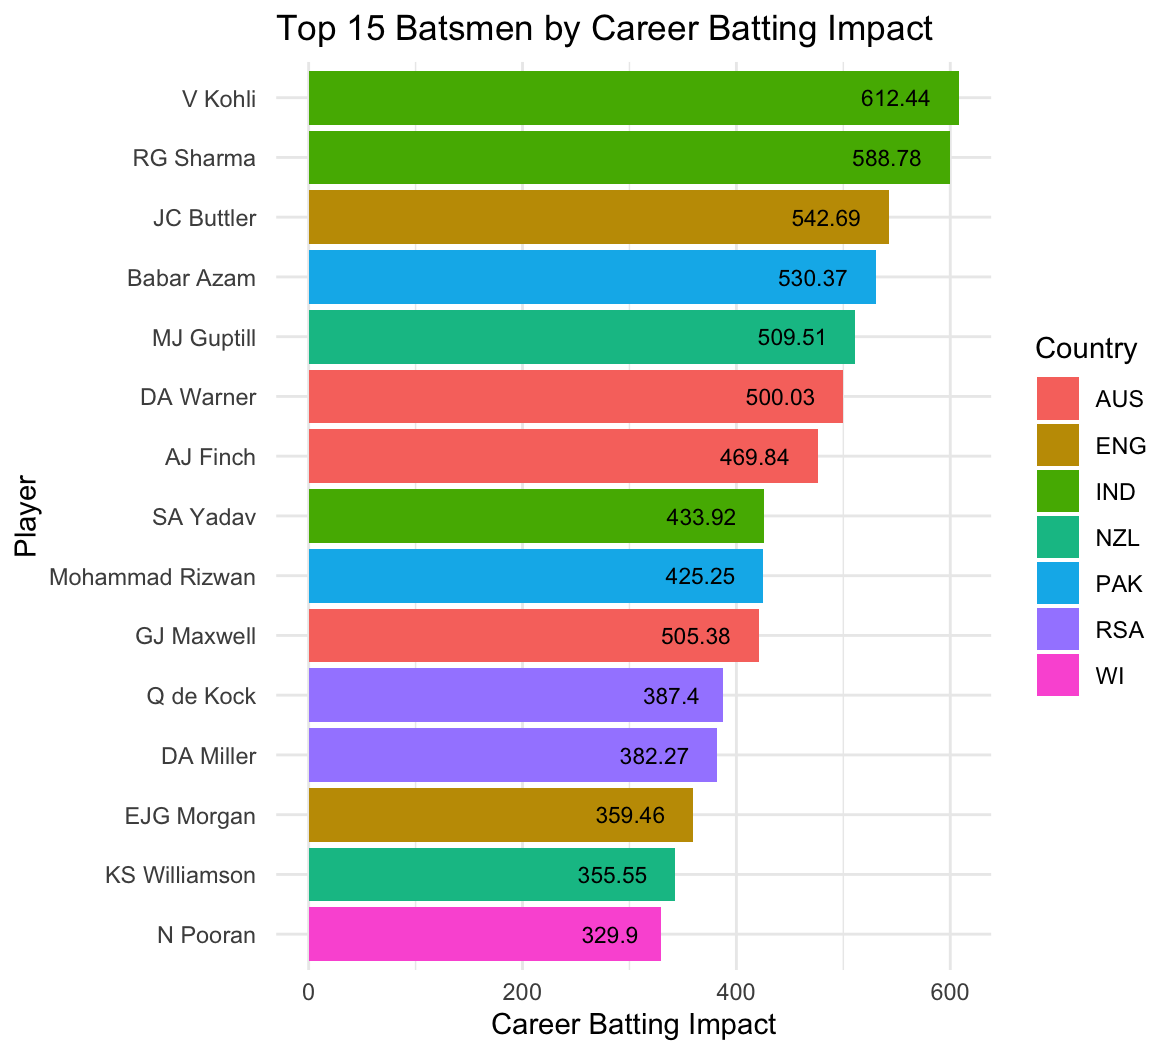
\includegraphics[width=0.45\linewidth]{bat_careerimpact.png} }}%
    \qquad
    \subfloat[\centering Bowling Career Impact]{{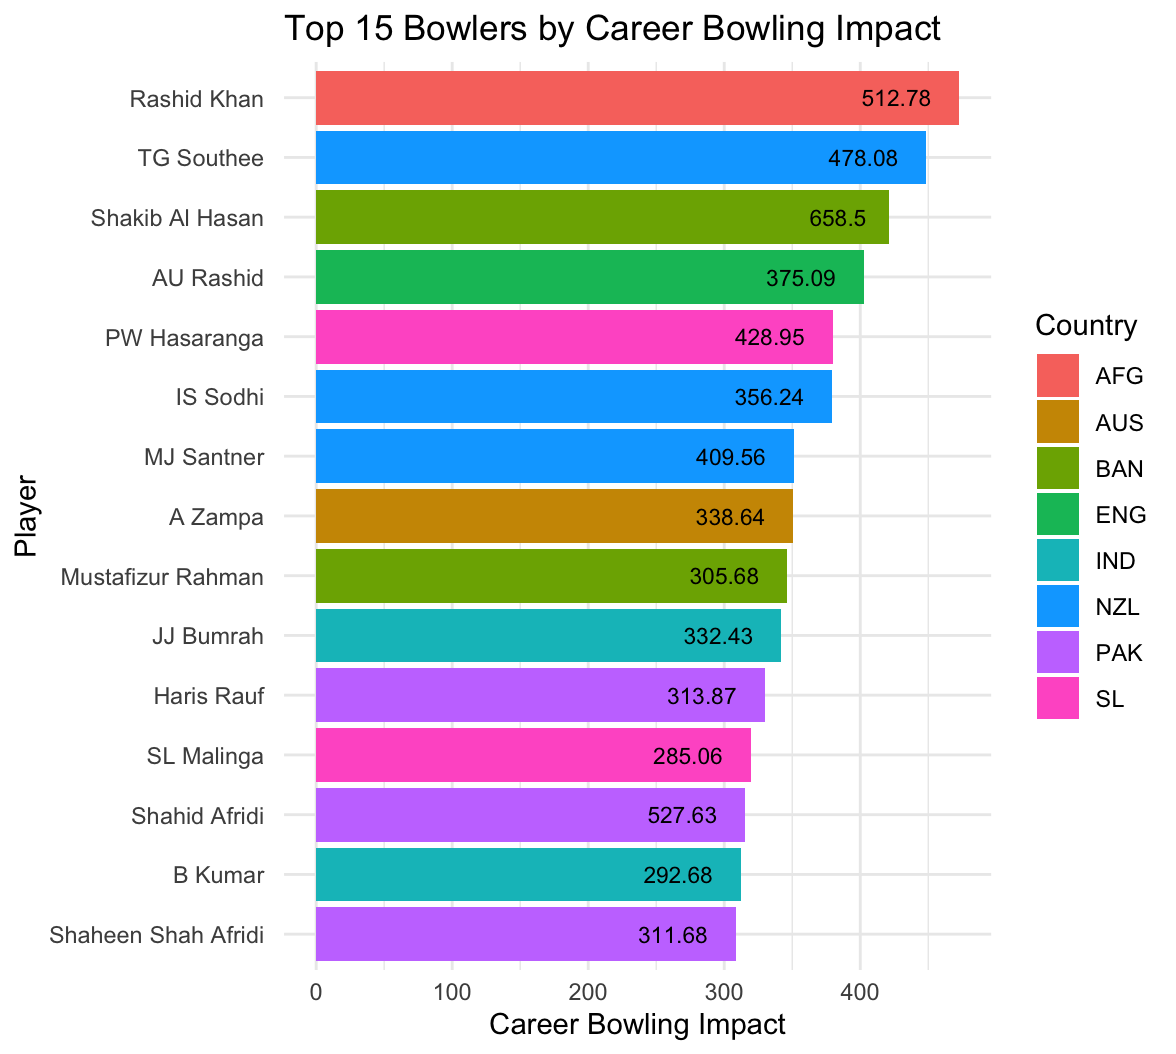
\includegraphics[width=0.45\linewidth]{bowl_careerimpact.png} }}%
    \caption{Total Career Bat/Bowl Impact Top 15}%
    \label{fig:career}%
\end{figure}

\begin{figure}[!htb]
    \centering
    \subfloat[\centering Batting Impact by game]{{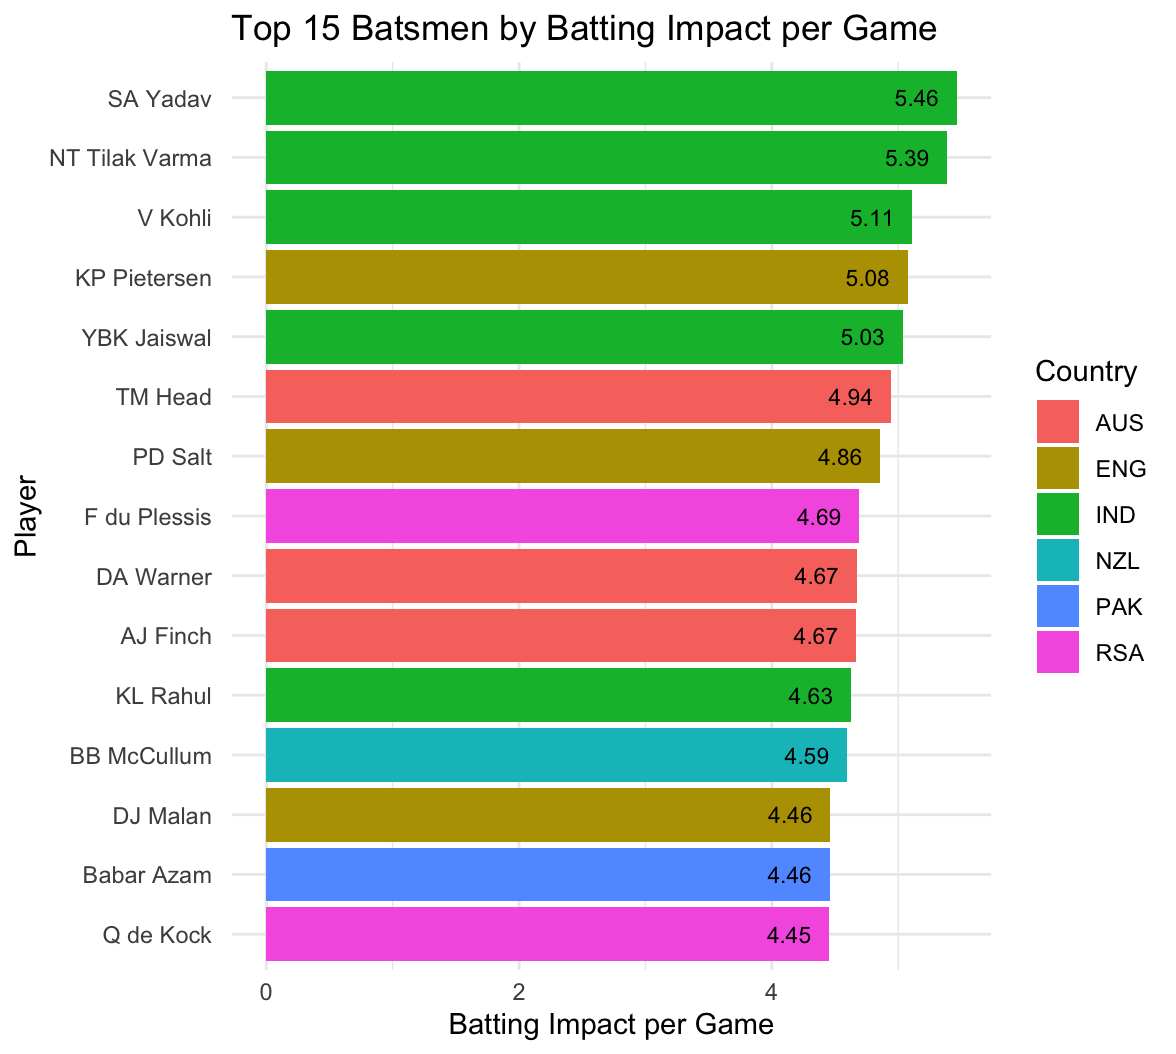
\includegraphics[width=0.45\linewidth]{batting_bygame.png} }}%
    \qquad
    \subfloat[\centering Bowling Impact by game]{{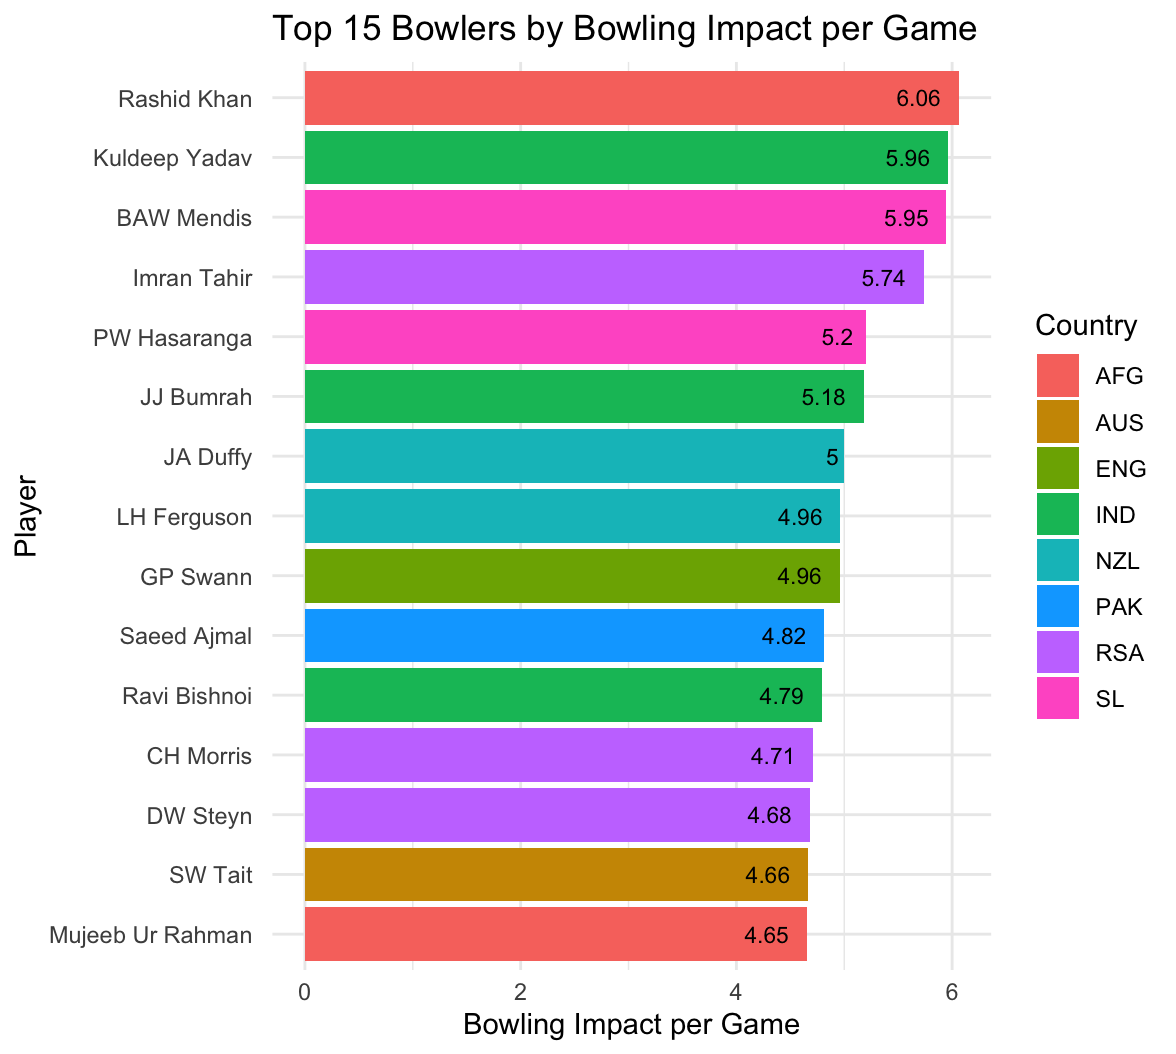
\includegraphics[width=0.45\linewidth]{bowling_bygame.png} }}%
    \caption{Bat/Bowl Impact Top 15 per game}%
    \label{fig:bygame}%
\end{figure}

\begin{figure}[!htb]
    \centering
    \subfloat[\centering All Rounder Total Impact]{{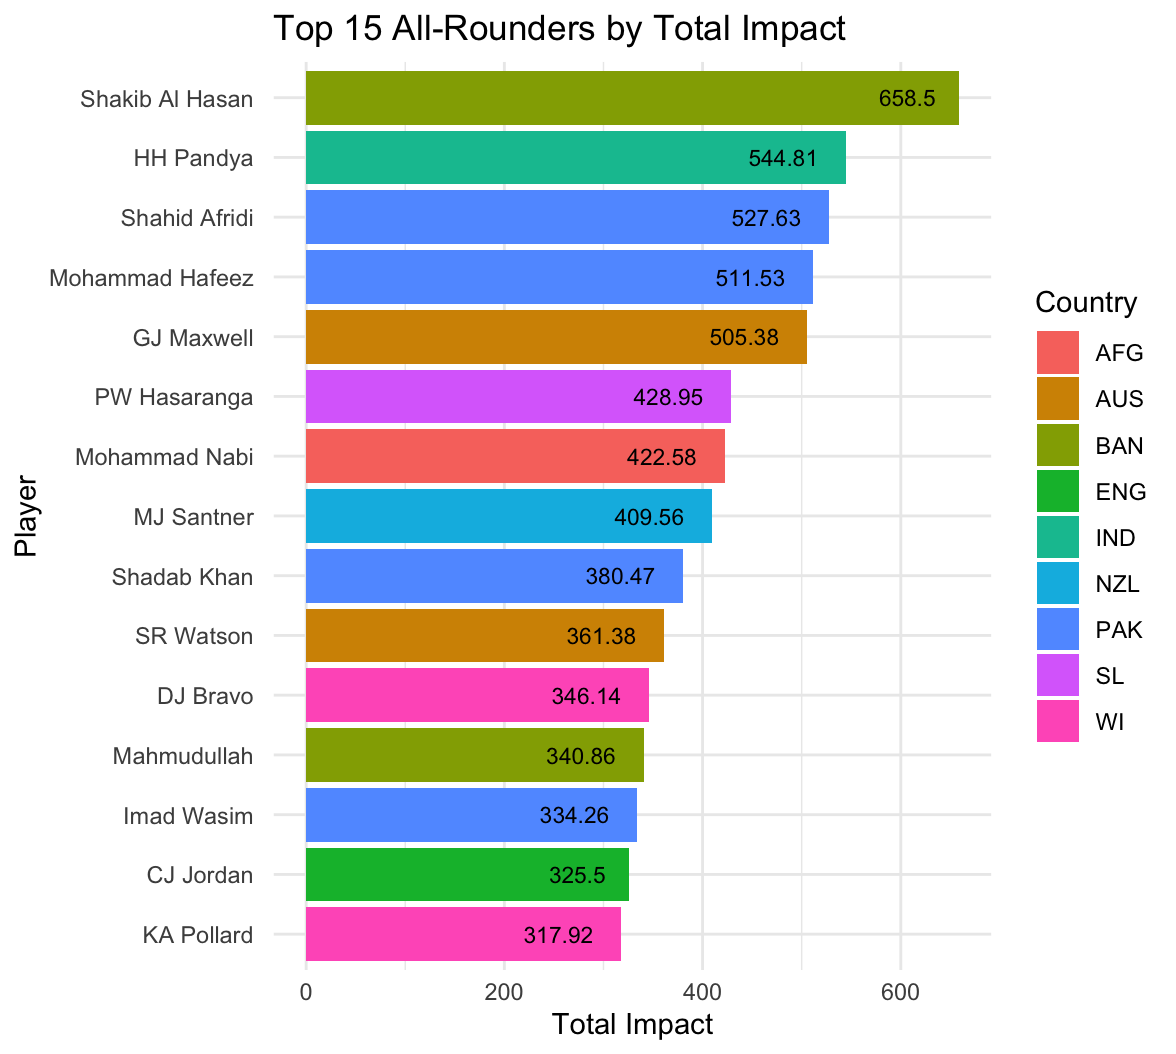
\includegraphics[width=0.45\linewidth]{allrounder_careerimpact.png} }}%
    \qquad
    \subfloat[\centering All Rounder Impact by game]{{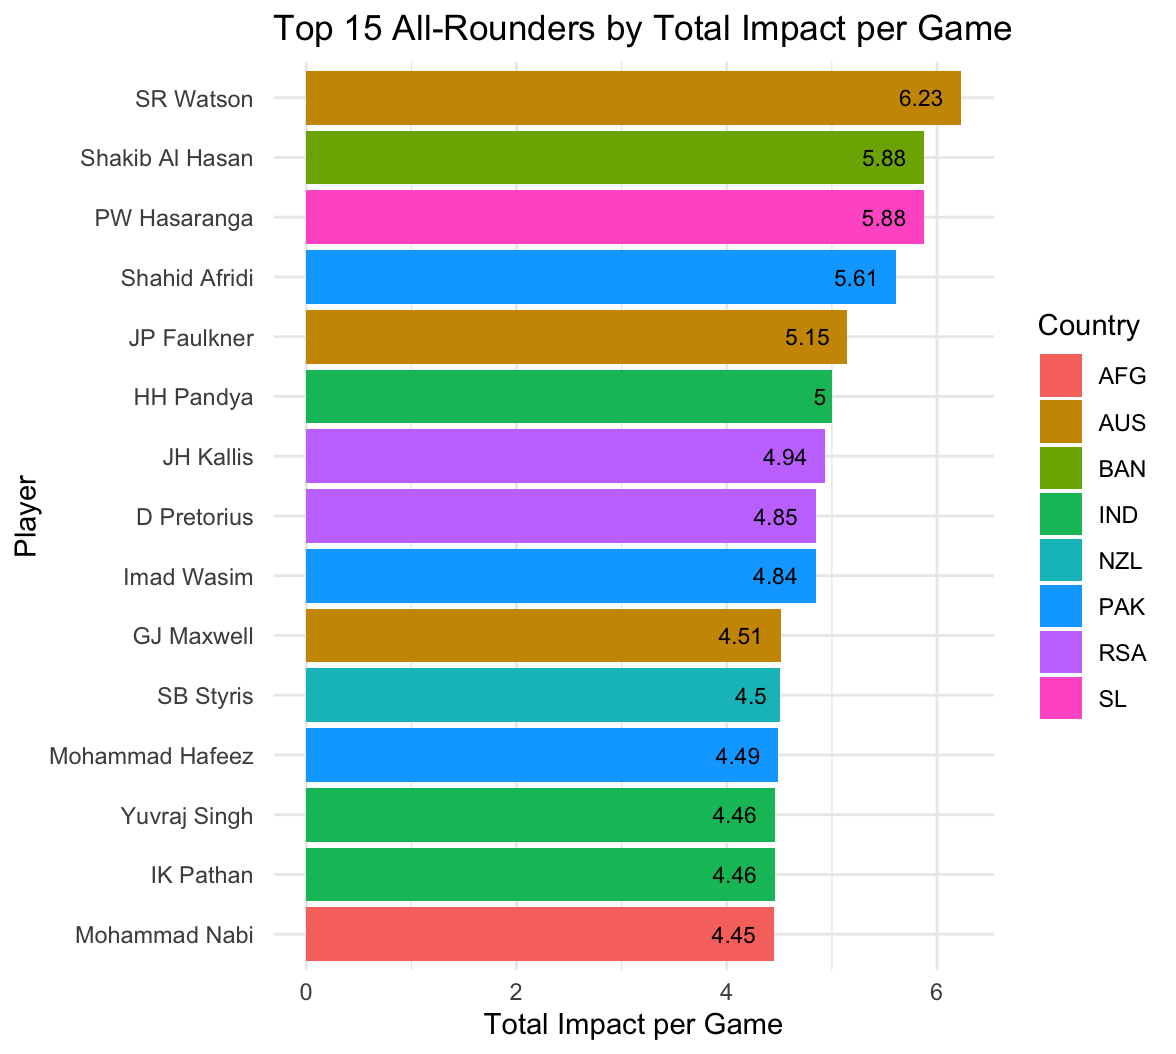
\includegraphics[width=0.45\linewidth]{allrounder_bygame.png} }}%
    \caption{All Rounder by game/career impact}%
    \label{fig:allround}%
\end{figure}

\begin{figure}[!htb]
    \centering
    \subfloat[\centering Best Bowling Venues]{{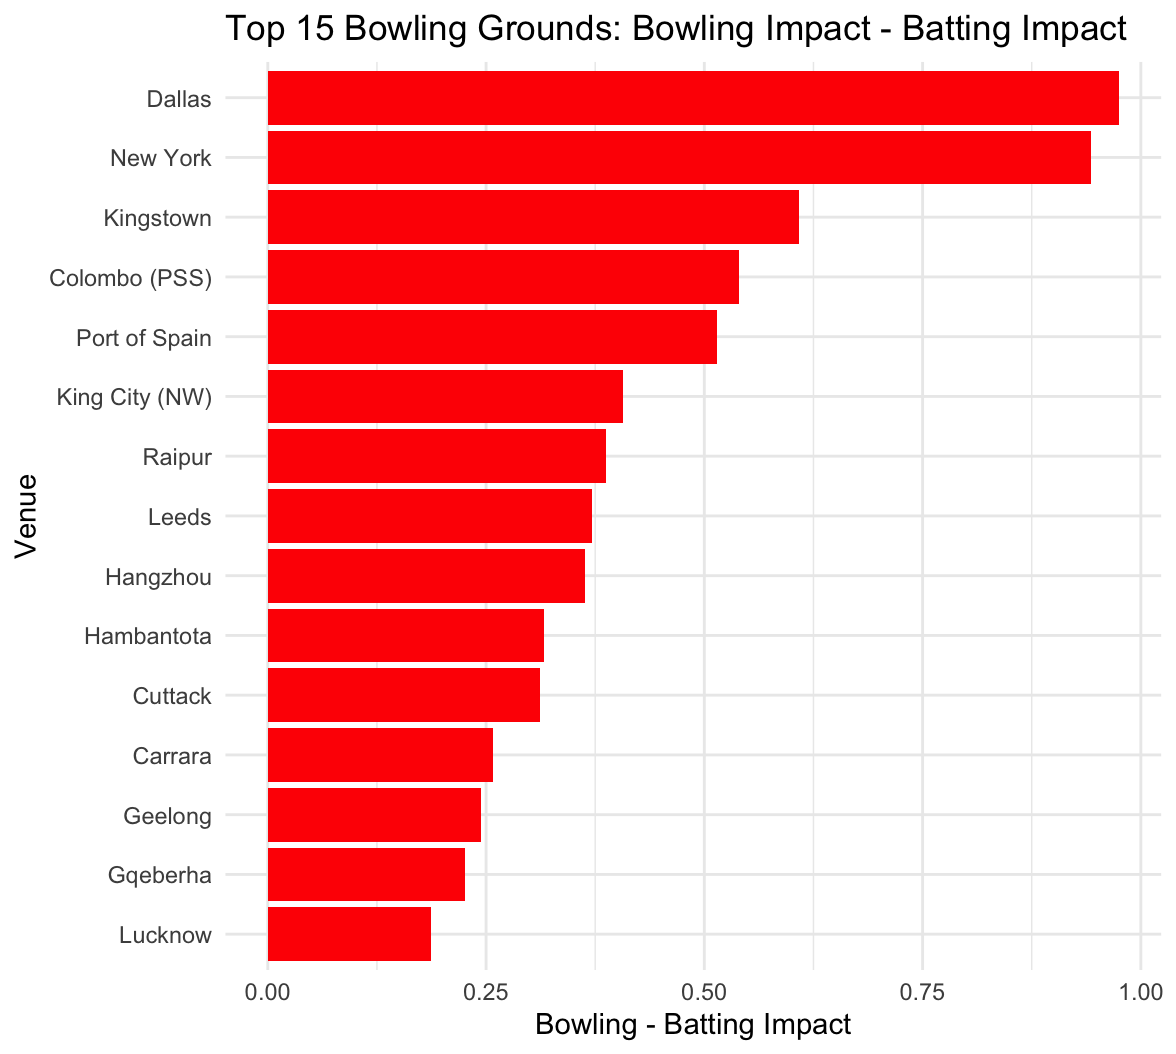
\includegraphics[width=0.45\linewidth]{Bowling_Grounds.png} }}%
    \qquad
    \subfloat[\centering Best Batting Venues]{{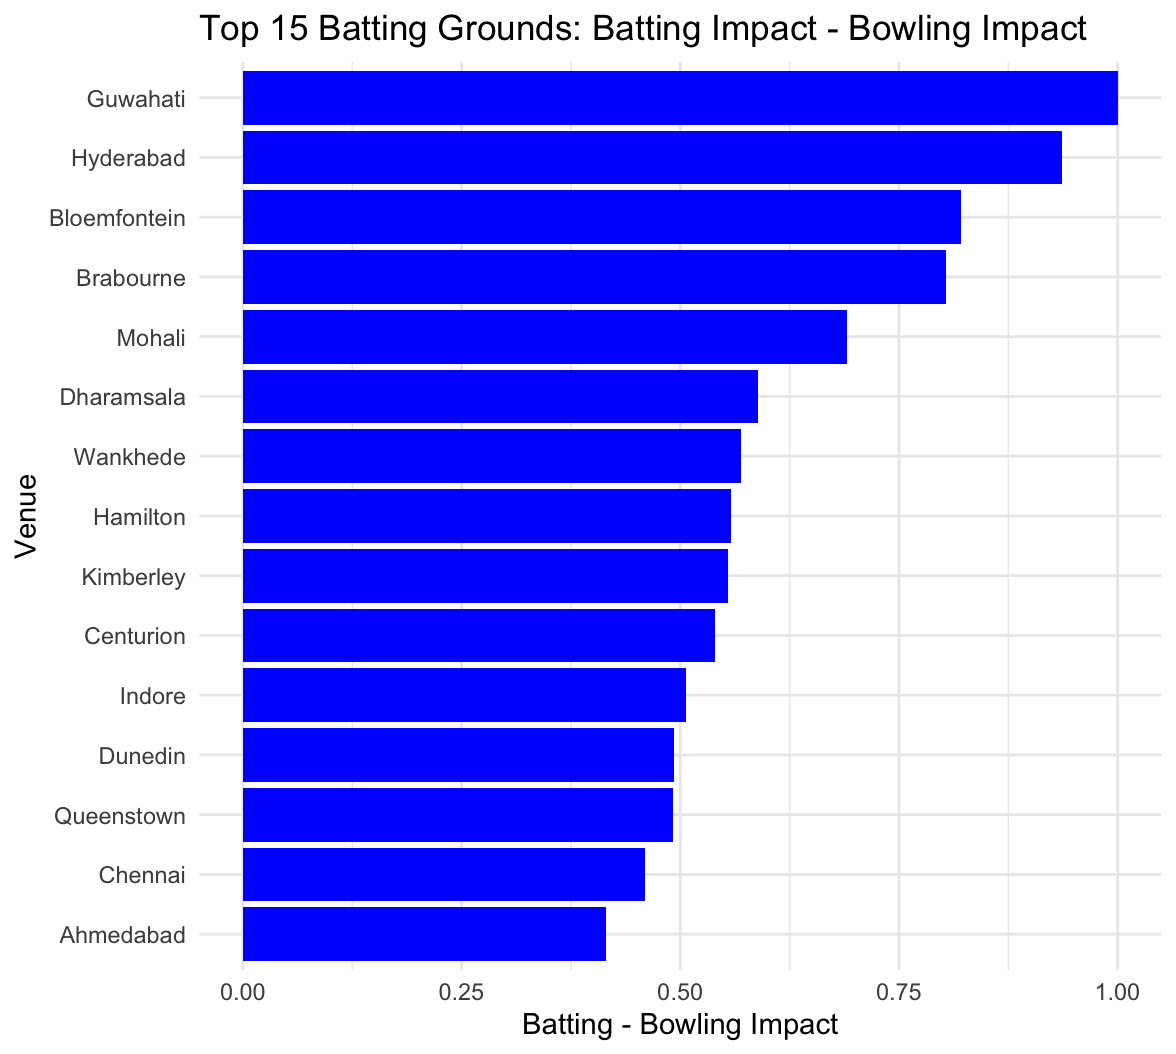
\includegraphics[width=0.45\linewidth]{Batting_Grounds.png} }}%
    \caption{Best Venues for Batting/Bowling}%
    \label{fig:venues}%
\end{figure}
\subsection{Code}
\label{appendix:vis1}
All code used to process data, generate figures, \& tune parameters/validate model at \\ \href{https://github.com/ArchithSharma/CricketPredictions}{https://github.com/ArchithSharma/CricketPredictions}. 
\clearpage
\section{Glossary of Cricket Terms Used}

\label{appendix:terms}


\subsection*{Batting Terms}
\begin{description}
  \item[Runs] Total number of runs scored by a batsman.
  \item[Strike Rate] The average number of runs scored per 100 balls faced. A higher strike rate indicates more aggressive scoring.
  \item[Boundary] A scoring shot that results in four (4) or six (6) runs.
  \item[Fours \& Sixes] A four occurs when the ball crosses the boundary after touching the ground; a six is when it crosses without touching the ground.
  \item[Batting Impact Score] A custom metric combining runs, strike rate, and boundaries to evaluate batting effectiveness.
  \item[Top Order] The group of batsmen who come out to bat first and score most of the runs, typically the first three or four guys in.
  \item[Middle Order] The group of batsmen that are typically all-rounders and power hitters to try and get quick runs near the end.
\end{description}

\subsection*{Bowling Terms}
\begin{description}
  \item[Wickets] The number of batsmen a bowler dismisses.
  \item[Maiden Overs] Overs in which no runs are conceded.
  \item[Economy Rate] Runs conceded per over bowled. A lower economy indicates more efficient bowling.
  \item[Spinner] A bowler who bowls slow but gets the ball to turn, deceiving batsmen.
  \item[Pacer] A bowler who bowls quick to try and beat batsmen with variations and leave them helpless.
  \item[Bowling Attack] The group of bowlers in a team and their combined effectiveness.
  \item[Bowling Impact Score] A weighted metric assessing bowling performance using wickets, maidens, and economy rate.
\end{description}

\subsection*{Match Context}
\begin{description}
  \item[T20I] Twenty20 International – a short-format cricket match where each team bowls a maximum of 20 overs.
  \item[Venue Factor] A numerical measure of how batting-friendly or bowling-friendly a stadium is, based on its average scoring.
  \item[Playing XI] The eleven players selected to participate in a match.
\end{description}

\subsection*{Strategy Terms}
\begin{description}
  \item[All-Rounder] A player who contributes significantly with both bat and ball.
  \item[Toss] The coin toss where the captain who wins decides whether to bat or bowl first.
  \item[Run rate] Runs per over (6 balls).
  \item[Pitch] Surface that the bowlers bowl to the batsmen on, can heavily influence team decisions by favoring batting or a certain kind of bowling.
  
  
\end{description}


\subsection*{Test playing nations list}
\label{appendix:list}
Afghanistan,
Australia,
Bangladesh,
England,
India,
Ireland,
New Zealand,
Pakistan,
South Africa,
Sri Lanka,
West Indies,
Zimbabwe.



\end{appendices}
\end{document}
